% vim: set spell:

\section{Formal Systems}

\begin{notion}

A formal system, $\mathcal{F}$, is a system of symbols and rules governing
their manipulation. A symbol of $\mathcal{F}$ is distinct from all other
symbols of $\mathcal{F}$.

\end{notion}

As such, the symbols of $\mathcal{F}$ form a set:

\begin{definition}

A set is a collection of distinct elements.

\end{definition}

Formal systems are a purely mental construct. To be used to any effect in the
material world, a formal system must be realised by a physical system.

\begin{notion}

A physical system, $\mathcal{P}$, is a system of physical symbols and processes
manipulating them. A symbol of $\mathcal{P}$ is physically distinct from all
other symbols of $\mathcal{P}$.

\end{notion}

Formal systems, and so their realisations, bear little intrinsic purpose ---
symbolic manipulation is a means to an end for more purposeful beings.
Consequently, a formal system may be more, or less reasonable for a particular
purpose; a physical system may be a more, or less reasonable realisation of a
particular formal system.

The reasonability of formal systems and their realisations is a matter to be
judged by the purposeful beings themselves. This text seeks to both present the
reader with various formal systems for various purposes, and to provide
transcripts of physical systems realising them. As such, some notational
matters are in order.

\begin{notation}

The elements of a set are typographically distinct symbols.

\end{notation}

\begin{notation}

Sets are denoted in one of two ways:

\begin{enumerate}[(1)]

\item By listing the elements in sequence, separated by commas, and enclosed in
braces.  For instance $\set{\symb{a},\symb{b},\symb{c}}$ denotes the set
containing (only) the elements $\symb{a}$, $\symb{b}$, and $\symb{c}$.

\item By exhibiting a procedure by which the elements can be listed in sequence
using paper and pencil.

\end{enumerate}

\end{notation}

To each consequent symbol in the sequence, we may assign a consequent

\begin{remark}

This representation of sets superimposes an order on the elements of a set. In
particular, the order of an element of the set, is position of the element in
the sequence.

\end{remark}

% any representation of a set demands us to put an ordering on the elements.

A physical system $\mathcal{P}$ is a reasonable realisation of a formal system
$\mathcal{F}$, provided that\begin{inparaenum}[(1)]\item there is a reasonable
correspondence between the symbols of $\mathcal{F}$ and the physical symbols of
$\mathcal{P}$, and \item $\mathcal{P}$ manipulates its physical symbols in
reasonable accordance with the rules of $\mathcal{F}$\end{inparaenum}. 

The process of symbolic manipulation may be transcribed to provide evidence
that the physical system is a reasonable realisation of a formal system.
Reasonability itself is judged by the purposeful beings, e.g. the readers of
this document.

Is a formal system


This demands a transcription of the definition of the formal system, compatible
with the transcription of a physical system.

This text seeks to both present the reader with various formal systems in mind of the author, and present transcriptions of physical systems 



In how
far a realisation is reasonable, is therefore a matter of the intended purpose
of the system.

The rules of $\mathcal{F}$ permit us to assess in how far $\mathcal{P}$ is a
reasonable realisation of $\mathcal{F}$ by means of physical processes.  As
such, formal systems are useful for communicating the intended (or perceived)
behaviour of physical systems.

This text presents both formal systems, and transcripts of physical systems
realising them. The reader is encouraged to further assess in how for the
physical realisations have been reasonable. As such, some matters of
typography are in order.

% For
% instance, the systems presented in this text are physical (typographical)
% realisations of the formal systems in mind of the author.

% Although this text does not 

For instance, this report is
(hopefully) a reasonable realisation of the formal systems in mind of the
author.

The reader is welcomed to evaluate the reasonability of the physical
realisations of the formal systems, by comparing them to their own physical
realisations.


The following definitions are made in the light that the formal systems in mind
of the author come to be realised as typographically in this text. The
definitions are made with a reader in mind.

\begin{definition}

A symbol of $\mathcal{F}$ is typographically distinct from all other symbols of
$\mathcal{F}$.

\end{definition}

As such, the symbols of $\mathcal{F}$ form a set. Denoted either as the listing
of symbols in a sequence, separated by commas and enclosed in braces, or by stating. For
instance $\set{a,b,c}$ denotes the set consisting of 3 distinct elements,
denoted $a$, $b$, and $c$.

\begin{definition}

A set is a collection of distinct elements.

\end{definition}

A symbol of $\mathcal{F}$ is distinguished from all other symbols of
$\mathcal{F}$. Similarly, a symbol of $\mathcal{P}$ is distinguished from all
other symbols of $\mathcal{P}$. As such, the symbols of $\mathcal{F}$ form a
set:

\begin{definition}

A set is a collection of distinct elements.

\end{definition}

An object of $\mathcal{F}$ is a combination of some symbols of
$\mathcal{F}$. For instance, given the symbols $a$, $b$, and $c$, we may
consider, among others, the following objects:

\begin{center}
$abc$
\quad\quad\quad
$\begin{matrix}
  & a &   \\
a & a & a \\
  & a &
\end{matrix}$
\quad\quad\quad
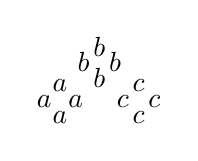
\begin{tikzpicture}
\draw (-0.5,0.0) node {$a$};
\draw (-0.7,0.2) node {$a$};
\draw (-0.3,0.2) node {$a$};
\draw (-0.5,0.4) node {$a$};
\draw (0.0,0.9) node {$b$};
\draw (0.2,0.7) node {$b$};
\draw (-0.2,0.7) node {$b$};
\draw (0.0,0.5) node {$b$};
\draw (0.5,0.0) node {$c$};
\draw (0.7,0.2) node {$c$};
\draw (0.3,0.2) node {$c$};
\draw (0.5,0.4) node {$c$};
\end{tikzpicture}

\end{center}

The rules of $\mathcal{F}$ enable us to make judgements about the objects of
$\mathcal{F}$. A judgement is a statement about some objects of $\mathcal{F}$,
which holds if it can be inferred from the rules of $\mathcal{F}$.  Judgements
come in various forms, judging over a number of objects. For instance, given
the objects $n$, $n_1$, and $n_2$, we may consider, among others, the following
forms of judgement:

\begin{table}[h]
\centering
\begin{tabular}{|l|l|}
\hline
\textbf{Judgement form} & \textbf{Reading} \\
\hline
$n\;\text{nat}$ & $n$ is a natural number. \\
\hline
$n=n_1+n_2$ & $n$ is the sum of $n_1$ and $n_2$.\\
\hline
\end{tabular}
\end{table}

% hypothetical judgement

The rules of $\mathcal{F}$ are rules of inference, dealing in judgements. A
rule is a relation between some judgements, called its premises, and a
judgement, called its conclusion\footnote{Although a set of premises may permit
us to infer multiple conclusions, we assume that they are inferred by different
rules.}. The rule, provided evidence that its premises hold, permits to infer
that the conclusion holds.

Let us adopt the common ``bar-notation'' for denoting rules, with the premises
of a rule presented above a horizontal line, and the conclusion below. For
instance, given the symbols $\symb{z}$ (read: zero) and $\symb{s}$ (read:
successor), we may consider the judgement $n\;\text{nat}$ to be defined as
follows:

\begin{equation}\label{natz-rules}
\sequent[NatZ-Zero]{}{\symb{z}\;\text{nat}}
\quad
\sequent[NatZ-Rec]{n\;\text{nat}}{{\symb{s}n\;\text{nat}}}
\end{equation}

Informally, these rules state that a natural number is either zero, or a
successor of a natural number.

Rules without premises are typically called axioms in that they hold
unconditionally. For instance, zero is always a natural number by the
\ruleref{Nat-Zero} axiom. The conclusion of one rule may form a premise of
another, perhaps the same, rule. This permits us to combine rule applications
into proofs of judgements. A proof is a witness that the judgement holds.

For instance, \ref{natz-rules} permits us to make the judgement
$\symb{s}\symb{s}\symb{s}\symb{z}\;\text{nat}$:

$$
\sequent{
  \sequent{
    \sequent{
      \sequent{
      }{\symb{z}\;\text{nat}}
    }{\symb{s}\symb{z}\;\text{nat}}
  }{\symb{s}\symb{s}\symb{z}\;\text{nat}}
}{\symb{s}\symb{s}\symb{s}\symb{z}\;\text{nat}}
$$

An object may be empty, that is, not consist of any symbols what-so-ever. For
instance, given some symbol $\bullet$ (read: star), we may consider the judgement
$n\;\text{nat}$ to be defined as follows:

\begin{equation}\label{nate-rules}
\sequent[NatE-Zero]{}{\;\text{nat}}
\quad
\sequent[NatE-Rec]{n\;\text{nat}}{\bullet n\;\text{nat}}
\end{equation}

Informally, these rules state that a natural number is either the empty object,
or a $\bullet$ followed by a natural number. Meaning that we can deduce which
natural number (in the classical sense) a natural number in $\mathcal{F}$
represents by counting the number of $\bullet$s. For instance, \ref{nate-rules}
permits us to make the judgement $\bullet\bullet\bullet\;\text{nat}$:

$$
\sequent{
  \sequent{
    \sequent{
      \sequent{
      }{\;\text{nat}}
    }{\bullet\;\text{nat}}
  }{\bullet\bullet\;\text{nat}}
}{\bullet\bullet\bullet\;\text{nat}}
$$

Empty objects can be a bit cryptic however, as they are not clearly
distinguished from other objects. It is convenient to adopt the following
notation:

\begin{definition}
Let $\varepsilon$ (read: epsilon) denote the empty object.
\end{definition}

\ref{nate-rules} can now be restated as follows:

\begin{equation}\label{nat-rules}
\sequent[Nat-Zero]{}{\varepsilon\;\text{nat}}
\quad
\sequent[Nat-Rec]{n\;\text{nat}}{\bullet n\;\text{nat}}
\end{equation}

Another informal reading of these rules is that a natural number is either the
empty sequence, or a sequence of $\bullet$s. Such a representation is
convenient as we can determine which natural number (in the classical sense)
$n\;\text{nat}$ represents by counting the number of $\bullet$s in $n$.

As another example, let the judgement $s\;\text{bitseq}$, reading $s$ is a
binary digit (bit) sequence, be defined as follows:

\begin{align}\label{bitseq-rules}
\begin{array}{c}
\sequent[BitSeq-Zero]{}{\varepsilon\;\text{bitseq}}
\\ \\
\sequent[BitSeq-Rec0]{s\;\text{bitseq}}{\symb{0} s\;\text{bitseq}}
\quad
\sequent[BitSeq-Rec1]{s\;\text{bitseq}}{\symb{1} s\;\text{bitseq}}
\end{array}
\end{align}

Informally, these rules state that a bit sequence is either the empty sequence,
or a sequence of bits (\symb{0} or \symb{1}).

The rules of \ref{nat-rules} and \ref{bitseq-rules} bear a lot of resemblance.
Both permit the sequencing of symbols chosen from an alphabet. Such sequencing
will be frequent throughout the thesis and so we define a generalized recursor
for it:

\begin{definition}

Given a judgement $w\;\Sigma$, let the judgement $s\;\Sigma^*$ be defined as
follows:

\begin{equation}\label{star-rules}
\sequent[Star-Zero]{}{\varepsilon\;\Sigma^*}
\quad
\sequent[Star-Rec]{
  w\;\Sigma \quad s\;\Sigma^*
}{
  w s\;\Sigma^*}
\end{equation}

\end{definition}

For instance, let $w\;\text{bullet}$ be defined as follows:

\begin{equation}
\sequent{}{\bullet\;\text{bullet}}
\end{equation}

\begin{theorem}
$s\;\text{bullet}^* \Leftrightarrow s\;\text{nat}$.
\end{theorem}

\begin{proof} Each direction by induction on the structure of $s$.. \end{proof}

Similarly, let $w\;\text{bit}$ be defined as follows:

\begin{equation}
\sequent{}{\symb{0}\;\text{bit}}
\quad
\sequent{}{\symb{1}\;\text{bit}}
\end{equation}

\begin{theorem}
$s\;\text{bit}^* \Leftrightarrow s\;\text{bitseq}$.
\end{theorem}

\begin{proof} Each direction by induction on the structure of $s$.. \end{proof}

Next: for each $s\;\Sigma^*$, there is a unique $n\;\text{nat}$ (recursive
enumerability).

\newpage

% The rules of a formal system may fall into a number of different classes. The
% class of \textbf{formation rules} consists of the rules governing how we can
% combine the symbols of the system to form \textbf{formulas}. The rest of the
% rules

% reasonably verifiable

% formal systems allow to state a problem
% the rules of a formal system allow to solve the problem

Formal systems are a purely mental construct. To be used to any effect in the
material world, a formal system must be realised by a physical system.

% Within our current understanding of the physical world, formal systems are an
% idealised construct. A \textbf{physical system} is subject to the laws of
% physics and other real-world constraints. Formal systems enjoy the freedom of
% the immaterial world.

% formal systems are specifications such that not only are they reasonably
% realisable, but also the adherence of the realisation to the specification is
% reasonably verifiable.

\begin{notion}

A physical system, $\mathcal{P}$, is a system of physical symbols and processes
manipulating them.

\end{notion}

$\mathcal{P}$ can be a reasonable realisation of formal system $\mathcal{F}$,
provided that\begin{inparaenum}[(1)]\item there is a reasonable correspondence
between the symbols of $\mathcal{F}$ and the physical symbols of $\mathcal{P}$,
and \item $\mathcal{P}$ manipulates the physical symbols in reasonable
accordance with the rules of $\mathcal{F}$\end{inparaenum}. For instance, this
report is (hopefully) a reasonable realisation of the formal systems that the
author had in mind.

If $\mathcal{P}$ is a reasonable realisation of $\mathcal{F}$, $\mathcal{F}$
can serve to specify the desired (or perceived) behaviour of $\mathcal{P}$.
Such a specification becomes useful in communicating how a physical system is
to be employed to solve a real-world problem.

\begin{notion}

$\mathcal{F}$ \textbf{solves} a problem $P$, if $P$ can be stated as formula
$f$ in $\mathcal{F}$, and after a finite sequence of symbolic manipulations
legal for $\mathcal{F}$, we arrive at a formula $f'$, which can be deemed a
statement of a solution to $P$.

\end{notion}

\pagebreak

Formal systems, and so their realisations, bear little intrinsic purpose ---
symbolic manipulation is a means to an end for more purposeful beings. In how
far a realisation is reasonable, is therefore a matter of the intended
\textbf{purpose} of the system.

\begin{notion}

A formal system $\mathcal{F}$ can solve a \textbf{problem} $P$, if $P$ can be
expressed with the symbols of $\mathcal{F}$, in accordance to the rules of
$\mathcal{F}$, 

\end{notion}

A system specification is useful to more purposeful beings for communicating
how a system can be used to solve a particular problem. The class of problems
which can be solved by rote symbolic manipulation is the class of
\textbf{computable} problems.

\begin{definition}

A problem is \textbf{computable} if it can be solved by performing a sequence
of symbolic manipulations.

\end{definition}

\begin{definition}

A \textbf{derivation} is a sequence of rule applications.

\end{definition}

\newpage

Formal
systems in this regard, become useful in communicating how a physical system is
to be used to solve a particular problem.


Physical systems realising formal systems are often referred to as
\textbf{computers}, and the activity of symbolic manipulation as
\textbf{computation}.

Before the mid-20th century, computation was generally the faculty of human
beings, with the help of paper and pencil, and perhaps, an abacus. With the
whirlwind of world history, human realisation of formal systems became
unreasonable, and we turned to computation by machines, less prone to err,
defect, or betray, and much faster at it.

This has allowed us to deal in a range of formal systems which we can
reasonably assume to be \textbf{absolutely realisable}, i.e. having physical
realisations which do not deviate from their formal specification. For
instance, we can reasonably assume that the Intel(R) Core(TM) i7-4600U
processor performs computation in accordance with its data sheet.

Dealing in absolutely realisable formal systems directly has proven a challenge
however.

As formal systems are a means to an end for more purposeful beings, we are not
only concerned with employing a formal system, 

This turn allowed for an elevation from much concern about physical
realisation, and today we generally assume that modern computers absolutely
realise the formal systems that specify them. As a result, the field of
Computer Science is generally concerned with\begin{inparaenum}[(1)]\item what
can be solved using formal systems, with \textbf{reasonable elegance} \item,
while \item staying within the realm of reasonable
realisability\end{inparaenum}.

To comply with (3), ... 

Much like a physical system can realise a formal system, a formal system
$\mathcal{G}$ can realise a formal system $\mathcal{F}$. This is usually
referred to as a \textbf{simulation}.

\begin{definition}

A formal system $\mathcal{F}=\chev{\mathcal{F}_S,\mathcal{F}_R}$ can be
simulated by a formal system $\mathcal{G}=\chev{\mathcal{G}_S,\mathcal{G}_R}$,
provided that\begin{inparaenum}[(1)]\item there is a 1-1 correspondence between
the $\mathcal{F}_S$ and $\mathcal{G}_S'$, where
$\mathcal{G}_S'\subseteq\mathcal{G}_S$, and \item $\mathcal{G}_R$ allow to
manipulate $\mathcal{G}_S'$ in accordance with $\mathcal{F}_R$\end{inparaenum}.

\end{definition}

% Desired for the formal system: consistent & complete
% Desired for the physical system: reliable, i.e. accurate.



